\documentclass{beamer}

\usepackage[utf8]{inputenc}
\usepackage[T1]{fontenc}
\usepackage[ngerman]{babel}
\usepackage{graphicx} % Bilder
\usepackage{wrapfig} % Umflussbilder
\usepackage{multicol} % Multiple columns
\usepackage{minted} % Haskell source code
\usepackage{framed} % Frames around source code
\usepackage[framemethod=tikz]{mdframed} % Frames
\usepackage{verbatim} % \begin{comment}...\end{comment}
\usepackage{etoolbox} % manipulate minted
\AtBeginEnvironment{minted}{\fontsize{10}{10}\selectfont}
\AfterEndEnvironment{minted}{}

\mdfdefinestyle{fancy}{
  roundcorner=5pt,
  linewidth=4pt,
  linecolor=red!80,
  backgroundcolor=red!20
}
\newmdenv[style=fancy]{important}

% redifine \em for \emph to use bold instead of italics
\makeatletter
\DeclareRobustCommand{\em}{%
  \@nomath\em \if b\expandafter\@car\f@series\@nil
  \normalfont \else \bfseries \fi}
\makeatother

% Stuff for Beamer
\beamertemplatenavigationsymbolsempty
\usetheme{Warsaw}

\title{Fortgeschrittene Funktionale Programmierung in Haskell}

\begin{document}
  
%----------------------------------------------------------------------------------------  

  \begin{frame}
  \begin{center}
    \huge\textbf{Fortgeschrittene Funktionale Programmierung in Haskell}\\ \bigskip
    \LARGE Universität Bielefeld, Sommersemester 2015\\ \bigskip
    \large Jonas Betzendahl \& Stefan Dresselhaus
    \end{center}
  \end{frame}

%----------------------------------------------------------------------------------------  
\begin{frame}[allowframebreaks]{Outline}
Übersicht für Heute:\smallskip

\tableofcontents
\end{frame}

%----------------------------------------------------------------------------------------
\section{Lens}
\subsection{Grundidee}
%----------------------------------------------------------------------------------------

\begin{frame}

\begin{center}
\Large
\textbf{Lenses}
\end{center}

\end{frame}

%----------------------------------------------------------------------------------------

\begin{frame}

\texttt{Lens} ist eine Bibliothek, geschrieben von Edward Kmett, einem 
Ikon der \texttt{Haskell}-Community. \texttt{Lens}es sind in vielen 
größeren Projekten nahezu unersätzlich und werden euch auf jeden Fall noch
häufiger begegnen, wenn ihr weiter \texttt{Haskell} macht.
\bigskip

\begin{center}
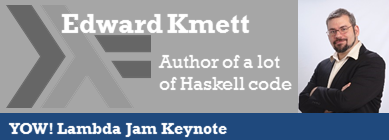
\includegraphics[scale=1]{kmett.png} 
\end{center}

\end{frame}

%----------------------------------------------------------------------------------------

\begin{frame}

\Large
Regel 1: Keine Panik!
\normalsize
\pause

\begin{multicols}{2}

\begin{center}
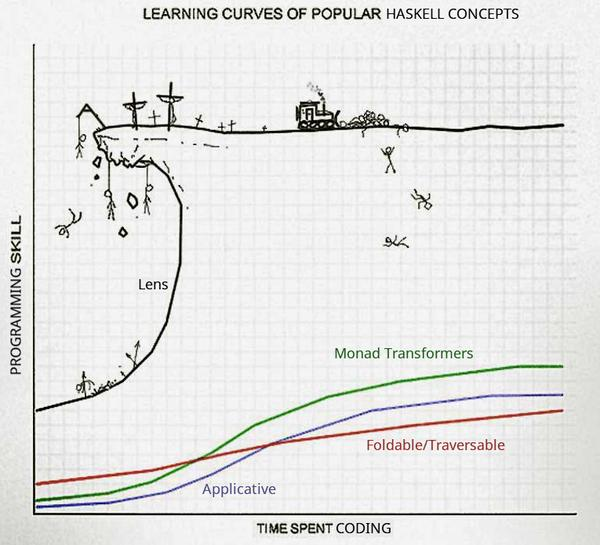
\includegraphics[scale=0.25]{learning_curve.jpg} 
\end{center}

\columnbreak
\quad


Sich über die Komplexität der \texttt{Lens}-Bibliothek lustig zu machen, ist zu einem gewissen \emph{inside joke} der Community geworden\dots
\pause
\bigskip

Das bedeutet aber auch, dass es (größtenteils) nicht so schlimm ist, wie Leute behaupten.

\end{multicols}

\end{frame}

%----------------------------------------------------------------------------------------

\begin{frame}[fragile]

\Large \textbf{\underline{Die Grundidee:}}\normalsize
\bigskip

Eine \texttt{Lens} gibt Zugriff auf einen bestimmten Teil eines Container oder einer sonstigen Datenstruktur.\pause\smallskip

Zugriff bedeutet hier\dots
\begin{itemize}
\item lesen, schreiben, modifizieren\dots\pause
\item aber auch falten, traversieren usw.\pause
\end{itemize}
\smallskip

\texttt{Lens}es sind \glqq first-class values\grqq\ (können also umhergereicht, in Datenstrukturen gepackt oder zurückgegeben werden\dots). Die simple Variante hat den Typ \texttt{Lens' s a}.
\pause
\bigskip

Beispiele:
\begin{verbatim}
  Lens' DateTime Hour
  Lens' DateTime Minute
  ...
\end{verbatim}
\end{frame}

%----------------------------------------------------------------------------------------

\begin{frame}

\Large \textbf{\underline{Die Grundidee:}}\normalsize

\begin{center}
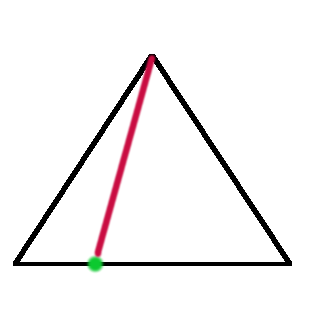
\includegraphics[scale=0.5]{lens_0.png} 
\end{center}

\end{frame}

%----------------------------------------------------------------------------------------

\begin{frame}

\Large \textbf{\underline{Die Grundidee:}}\normalsize

\begin{center}
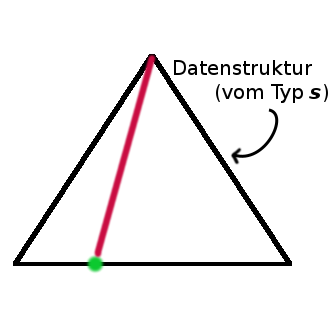
\includegraphics[scale=0.5]{lens_1.png} 
\end{center}

\end{frame}

%----------------------------------------------------------------------------------------

\begin{frame}

\Large \textbf{\underline{Die Grundidee:}}\normalsize

\begin{center}
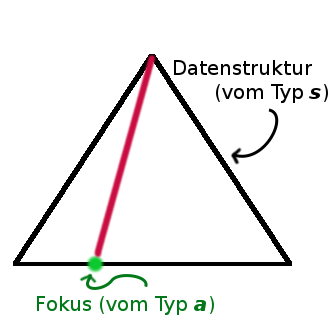
\includegraphics[scale=0.5]{lens_2.png} 
\end{center}

\end{frame}

%----------------------------------------------------------------------------------------

\begin{frame}

\Large \textbf{\underline{Die Grundidee:}}\normalsize

\begin{center}
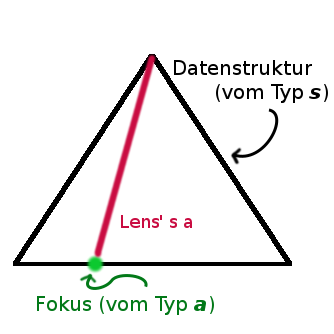
\includegraphics[scale=0.5]{lens_3.png} 
\end{center}

\end{frame}

%----------------------------------------------------------------------------------------

\begin{frame}[fragile]

\begin{multicols}{2}
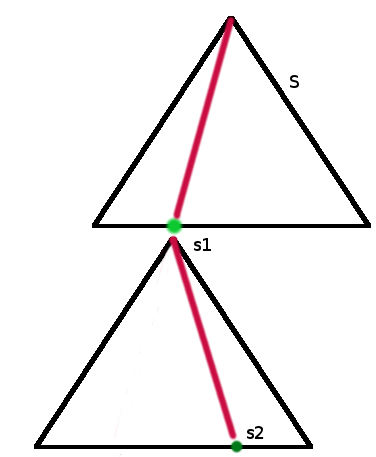
\includegraphics[scale=0.4]{lenses_compose.png} 

\columnbreak

Was wir gerne hätten: \texttt{Lens}es, die sich einfach miteinander kombinieren lassen.
\bigskip

\begin{minted}{haskell}
composeL :: Lens' s s1 
         -> Lens' s1 s2
         -> Lens' s s2
\end{minted}

Wir wissen bereits, dass Composability ein großer Vorteil für funktioniale Konstrukte ist.\smallskip

\glqq Puzzle Programming\grqq\ macht es uns einfacher, korrekte und elegante Programme zu schreiben.
\end{multicols}
\end{frame}

%----------------------------------------------------------------------------------------
\subsection{Motivation \& Anwendungen}
%----------------------------------------------------------------------------------------

\begin{frame}[fragile]

Aber warum brauchen wir sowas? Geht das nicht alles schon mit Pattern-Matching?
\pause

\begin{minted}{haskell}
data Person = Person { name :: String
                     , addr :: Address }
                     
data Address = Address { road :: String
                       , city :: String
                       , pstc :: Int }
                       
setName :: String -> Person -> Person 
setName nm p = p { name = nm } -- record update notation

setPostcode :: Int -> Person -> Person
setPostcode pc p = p { addr = addr p { pstc = pc } }
\end{minted}

Ja, das geht. Aber es wird schnell ermüdend. Wer beim Erklären zu oft \glqq blah-blah\grqq\ sagt, sollte sich um elegantere Wege oder Automatisierung bemühen.

\end{frame}

%----------------------------------------------------------------------------------------

\begin{frame}[fragile]

Angenommen, wir hätten jetzt eine \texttt{Lens} für jedes Feld, \dots

\begin{minted}{haskell}
lname :: Person -> String
laddr :: Person -> Address
\end{minted}
\pause

\dots Funktionen, die \texttt{Lens}es zum lesen und schreiben benutzen, \dots

\begin{minted}{haskell}
view :: Lens' s a -> s -> a
set  :: Lens' s a -> a -> s -> s
\end{minted}
\pause

\dots dann könnten wir (zusammen mit der \texttt{composeL}-Funktion) deutlich eleganteren und effizienteren Code schreiben:\bigskip

\begin{minted}{haskell}
setPostcode :: Int -> Person -> Person
setPostcode pc p = set (laddr `composeL` lpstc) pc p
\end{minted}

\end{frame}

%----------------------------------------------------------------------------------------

\begin{frame}[fragile]

Der naive Ansatz für so eine Struktur wäre wahrscheinlich, einfach feste Getter und Setter zu bündeln:

\begin{minted}{haskell}
data LensR s a = L { view :: s -> a
                   , set  :: a -> s -> s }
\end{minted}
\pause

Mit etwas Hirnschmalz kriegen wir sogar \texttt{composeL}:

\begin{minted}{haskell}
composeL :: LensR s s1 -> LensR s1 s2 -> LensR s s2
composeL (L v1 u1) (L v2 u2) = L (\s -> v2 (v1 s))
                                 (\a s -> u1 (u2 a (v1 s)) s) 
\end{minted}
\pause
\dots all das ist aber sehr ineffizient. Falls wir \texttt{over} haben wollen

\mint{haskell}|over :: Lens s a -> (a -> a) -> s -> s|

\dots müssten wir erst getten, dann setten. \emph{Nicht cool}.

\end{frame}

%----------------------------------------------------------------------------------------

\begin{frame}[fragile]

Wir könnten jetzt einfach eine \texttt{modify}-Funktion hinzufügen:

\begin{minted}{haskell}
data LensR s a = L { view   :: s -> a
                   , set    :: a -> s -> s 
                   , modify :: (a -> a) -> s -> s }
\end{minted}
\pause

Das Problem dabei ist nur, dass wir sehr schnell zu viele Funktionen haben. Was ist mit
effektvollen Veränderungen? Oder mit Veränderungen, die Fehlschlagen können?
\pause

\begin{minted}{haskell}
data LensR s a =
    L { view        :: s -> a
      , set         :: a -> s -> s 
      , modify      :: (a -> a) -> s -> s 
      , modidyIO    :: (a -> IO a) -> s -> IO s
      , modifyMaybe :: (a -> Maybe a) -> s -> Maybe s }
\end{minted}

Diese Datenstruktur wächst uns schnell über den Kopf und ist dafür nicht mal sehr flexibel.

\end{frame}

%----------------------------------------------------------------------------------------

\begin{frame}

\begin{center}

\includegraphics[scale=1]{the-end-or-is-it.jpg} 
\end{center}

\end{frame}

%----------------------------------------------------------------------------------------

\begin{frame}[fragile]
Das geübte Auge findet zumindest für den letzten Schritt noch einen Ausweg.
\pause

Wir könnten immerhin die Funktionen \texttt{modifyMaybe} und \texttt{modifyIO} (und alle, die dem gleichen Muster folgen) zusammenfassen:

\begin{minted}{haskell}
data LensR s a =
    L { view    :: s -> a
      , set     :: a -> s -> s 
      , modify  :: (a -> a) -> s -> s 
      , modidyF :: Functor f => (a -> f a) -> s -> f s }
\end{minted}

Und das ist eine wirklich gute Idee. 

\end{frame}

%----------------------------------------------------------------------------------------

\begin{frame}[fragile]

\textbf{Edward's big insight:}
\pause
\smallskip

Eine \emph{noch} bessere Idee ist es allerdings (und das ist die große Idee hinter \texttt{Lens}), auch die Funktionen \texttt{view}, \texttt{set} und \texttt{modify} über die Funktion \texttt{modifyF} auszudrücken!
\pause
\smallskip\smallskip

\begin{minted}{haskell}
type Lens' s a = forall f. Functor f => (a -> f a) -> s - > f s
\end{minted}
\pause
\smallskip\smallskip

Das ist nur noch ein \texttt{type}, also ein Alias von einem Typen auf einen anderen. Mehr brauchen wir nicht.

\end{frame}

%----------------------------------------------------------------------------------------

\begin{frame}[fragile]

\textbf{Fun Fact:} \texttt{Lens'} und \texttt{LensR} sind \emph{isomorph}!
\pause
\smallskip\smallskip

Das bedeutet wir können folgende Funktionen schreiben:

\begin{minted}{haskell}
lensR2Lens :: LensR s a -> Lens' s a
lens2LensR :: Lens' s a -> LensR s a
\end{minted}
\pause

Hier werden wir eine Richtung vortanzen, die andere Richtung ist Übungsaufgabe. ;-)

\begin{minted}{haskell}
set :: Lens' s a -> (a -> s -> s)
set ln a s = ... aehm ...
\end{minted}
\pause

\texttt{ln}, wenn angewendet, gibt irgendein \texttt{f s} zurück, wir wollen aber eigentlich nur ein \texttt{s}. \pause
Also müssen wir uns ein passendes \texttt{f} wählen:

\begin{minted}{haskell}
newtype Identity a = Identity a

runIdentity :: Identity a -> a 
runIdentity (Identity x) = x

instance Functor Identity where
   fmap f (Identity s) = Identity (f s)
\end{minted}
 
\end{frame}

%----------------------------------------------------------------------------------------

\begin{frame}[fragile]

\textbf{Fun Fact:} \texttt{Lens'} und \texttt{LensR} sind \emph{isomorph}!
\smallskip\smallskip

Das bedeutet wir können folgende Funktionen schreiben:

\begin{minted}{haskell}
lensR2Lens :: LensR s a -> Lens' s a
lens2LensR :: Lens' s a -> LensR s a
\end{minted}

Hier werden wir eine Richtung vortanzen, die andere Richtung ist Übungsaufgabe. ;-)

\begin{minted}{haskell}
set :: Lens' s a -> (a -> s -> s)
set ln x s = runIdentity (ln set_fld s)
  where
    set_fld :: a -> Identity a
    set_fld _ = Identity x -- discard current
                           -- return new value x
\end{minted}
\end{frame}

%----------------------------------------------------------------------------------------

\begin{frame}[fragile]
\begin{overprint}
\onslide<1>
\begin{minted}{haskell}
view :: Lens' s a -> s -> a
view ln = ... aehm ...
\end{minted}
\onslide<2-3>
\begin{minted}{haskell}
view :: Lens' s a -> s -> a
view ln = ... aehm ...
\end{minted}
Wieder einmal gibt uns die \texttt{Lens} ein \texttt{f s} zurück, wir wollen aber 
einen Wert vom Typ \texttt{a}. WTF?
\onslide<4>
\begin{minted}{haskell}
view :: Lens' s a -> s -> a
view ln s = getConst (ln Const s) 
\end{minted}
\smallskip
Die Idee: Wir packen das \texttt{a} in das \texttt{f}.\\ \texttt{Const} hat hier den Typen \texttt{a -> Const a a}. Auf was wird also \texttt{f} instanziiert?
\end{overprint}
\vspace{0.3cm}
\begin{overprint}
\onslide<3->
Erinnerung:
\begin{minted}{haskell}
type Lens' s a = forall f. Functor f =>
                   (a -> f a) -> s -> f s
                   
newtype Const v a = Const v

getConst :: Const v a -> v
getConst (Const x) = x

instance Functor (Const v) where
    fmap f (Const x) = Const x
\end{minted}
\end{overprint}

\end{frame}

%----------------------------------------------------------------------------------------

\begin{frame}[fragile]

\textbf{Fun Fact:} \texttt{Lens'} und \texttt{LensR} sind \emph{isomorph}!
\smallskip\smallskip

Nach point-free-style umgeschrieben und zusammengesteckt:

\begin{minted}{haskell}
view :: Lens' s a -> s -> a
view ln = getConst . ln Const

set :: Lens' s a -> a -> s -> s
set ln x = getIdentity . ln (Identity . const x)

-- one way of the isomorphism
lens2LensR :: Lens' s a -> LensR s a
lens2LensR ln = L { viewR = view ln, setR = set ln }

-- the other way of the isomorphism
lensR2Lens :: LensR s a -> Lens' s a
lensR2Lens = error "ToDo"
\end{minted}
 
\end{frame}

%----------------------------------------------------------------------------------------
\subsection{Fortgeschrittenes}
%----------------------------------------------------------------------------------------

\begin{frame}[fragile]

Bisher haben wir uns nur angeschaut, wie wir \texttt{Lens}es benutzen. Wir wollen aber auch noch sehen, wie wir uns welche \emph{bauen} können.
\pause
\smallskip
\smallskip

Zur Erinnerung:
\begin{minted}{haskell}
type Lens' s a = forall f. Functor f =>
                   (a -> f a) -> s -> f s
\end{minted}
\pause
\smallskip

\begin{minted}{haskell}
-- field names with underscores so lenses can have the names
data Person = P { _name :: String, _balance :: Integer}
\end{minted}
\pause
\bigskip

\begin{minted}{haskell}
-- name :: Functor f => (String -> f String)
--                   -> Person  -> f Person
name :: Lens' Person String
.
\end{minted}

\end{frame}

%----------------------------------------------------------------------------------------

\begin{frame}[fragile]

Bisher haben wir uns nur angeschaut, wie wir \texttt{Lens}es benutzen. Wir wollen aber auch noch sehen, wie wir uns welche \emph{bauen} können.
\smallskip
\smallskip

Zur Erinnerung:
\begin{minted}{haskell}
type Lens' s a = forall f. Functor f =>
                   (a -> f a) -> s -> f s
\end{minted}
\smallskip

\begin{minted}{haskell}
-- field names with underscores so lenses can have the names
data Person = P { _name :: String, _balance :: Integer}
\end{minted}
\bigskip

\begin{minted}{haskell}
-- name :: Functor f => (String -> f String)
--                   -> Person  -> f Person
name :: Lens' Person String
name fn (P n b) = ... aehm ...
\end{minted}

\end{frame}

%----------------------------------------------------------------------------------------

\begin{frame}[fragile]

Bisher haben wir uns nur angeschaut, wie wir \texttt{Lens}es benutzen. Wir wollen aber auch noch sehen, wie wir uns welche \emph{bauen} können.
\smallskip
\smallskip

Zur Erinnerung:
\begin{minted}{haskell}
type Lens' s a = forall f. Functor f =>
                   (a -> f a) -> s -> f s
\end{minted}
\smallskip

\begin{minted}{haskell}
-- field names with underscores so lenses can have the names
data Person = P { _name :: String, _balance :: Integer}
\end{minted}
\bigskip

\begin{minted}{haskell}
-- name :: Functor f => (String -> f String)
--                   -> Person  -> f Person
name :: Lens' Person String
name fn (P n b) = fmap (\n' -> P n' b) (fn n)
\end{minted}
\pause

Mit etwas mentaler Gymnastik merken wir: Die Typen stimmen!

\end{frame}

%----------------------------------------------------------------------------------------

\begin{frame}[fragile]

Wir können genau diese \texttt{Lens} jetzt verwenden.
\pause

\begin{verbatim}
ghci> let fred = P { _name = "Fred", _balance = 1000 }
ghci> view name fred
"Fred"
ghci> set name "Bill" fred
P { _name = "Bill", _balance = 1000 }
\end{verbatim}
\pause

Aber wie funktioniert das genau?\pause

\begin{minted}{haskell}
ghci> view name P { _name = "Fred", _balance = 1000 }
      -- inline view
= getConst (name Const (P { _name = "Fred", _balance = 1000 }))
      -- inline name
= getConst (fmap (\n' -> P n' 1000) (Const "Fred"))
      -- fmap f (Const x) = Const x
= getConst (Const "Fred")
      -- getConst (Const x) = x
= "Fred"
\end{minted}

\end{frame}

%----------------------------------------------------------------------------------------

\begin{frame}[fragile]
\textbf{\texttt{Lens} laws:}
\smallskip

Wenn wir eigene \texttt{Lens}es bauen, müssen wir ein paar Regeln beachten. Dann wie bestimmte
Typklassen (\texttt{Functor, Applicative, Monad}), haben auch \texttt{Lens}es ihre eigenen Regeln.\pause
\bigskip

Glücklicherweise sind sie nicht sehr kompliziert:
\begin{itemize}
\item Man bekommt heraus, was man rein tut:\\
\mint{haskell}|view l (set l v s)  == v|
\pause
\item Zurücklegen was man bekam ändert nichts:\\
\mint{haskell}|set l (view l s) s  == s|
\pause
\item Zweimal setzen ist das gleiche wie einmal setzen:\\
\mint{haskell}|set l v' (set l v s) == set l v' s|
\end{itemize}

\end{frame}

%----------------------------------------------------------------------------------------

\begin{frame}[fragile]

\textbf{\texttt{Lens}es generieren lassen:}\smallskip

\begin{minted}{haskell}
data Person = P { _name :: String, _balance :: Integer}

name :: Lens' Person String
name fn (P n b) = fmap (\n' -> P n' b) (fn n)
\end{minted}

Jedes Mal alle Lenses von Hand zu schreiben, wenn wir einen Datentypen anlegen
wäre ziemlich schreibaufwändig. Aber genau davon wollen wir doch eigentlich weg.
\pause

Die Lösung: Statt dem Code oben können wir schreiben:

\begin{minted}{haskell}
import Control.Lens.TH
data Person = P { _name :: String, _balance :: Integer}

$(makeLenses ''Person)
\end{minted}
%$

So erstellt \texttt{TemplateHaskell} \texttt{Lens}es für \emph{alle} Felder. Danke, Edward Kmett. :D

\end{frame}

%----------------------------------------------------------------------------------------

\begin{frame}[fragile]

\begin{multicols}{2}
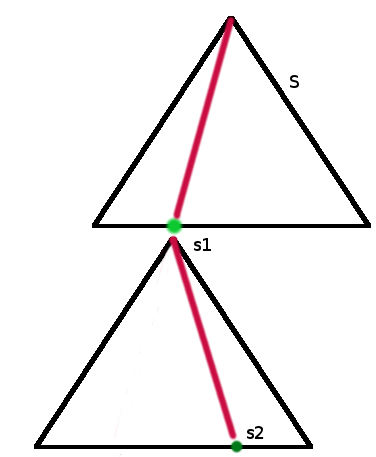
\includegraphics[scale=0.4]{lenses_compose.png} 

\columnbreak

\textbf{Lens composition:}\smallskip

Ihr erinnert euch: Wir wollten gerne eine Funktion \texttt{composeL} haben, mit der wir
zwei verschiedene \texttt{Lens}es aneinander kleben können. 

\begin{minted}{haskell}
composeL :: Lens' s s1 
         -> Lens' s1 s2
         -> Lens' s s2
\end{minted}

Glücklicherweise ist das dieses Mal kein großer Aufwand\dots

\pause

\textbf{Lens composition is just function composition!}

\end{multicols}
\end{frame}

%----------------------------------------------------------------------------------------

\begin{frame}[fragile]
Wir wollten auch gerne solche Funktionen in unseren \texttt{Lens}es haben wie \texttt{modifyMaybe} oder \texttt{modifyIO}.

\begin{minted}{haskell}
modifyMaybe :: Lens' s a -> (a -> Maybe a) -> s -> Maybe s
modifyIO    :: Lens' s a -> (a -> IO a) -> s -> IO a
\end{minted}
\pause

Total einfach! Eine \texttt{Lens} \emph{ist} schon so eine Funktion!

\begin{minted}{haskell}
type Lens' s a = forall f. Functor f =>
                   (a -> f a) -> s -> f s
\end{minted}

Und so sehen wir auch, dass es sinnig ist, \texttt{f} mit anderen Funktoren als \texttt{Const}
oder \texttt{Identity} zu instanziieren.

\end{frame}

%----------------------------------------------------------------------------------------
\subsection{Traversals}
%----------------------------------------------------------------------------------------

\begin{frame}[fragile]
\textbf{Edward's zweite große Einsicht:}\pause\bigskip

\begin{minted}{haskell}
type Lens' s a = forall f. Functor f =>
                   (a -> f a) -> s -> f s
\end{minted}

\begin{center}
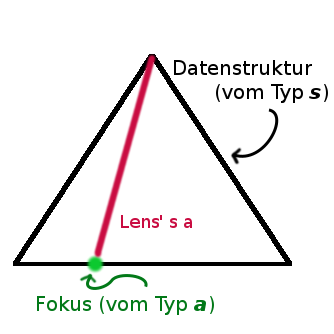
\includegraphics[scale=0.4]{lens_3.png} 
\end{center}
\pause

Was passiert, wenn wir statt \texttt{Functor} ein \texttt{Applicative} fordern?

\end{frame}

%----------------------------------------------------------------------------------------

\begin{frame}[fragile]
\textbf{Edward's zweite große Einsicht:}\bigskip

\begin{minted}{haskell}
type Traversal' s a = forall f. Applicative f => 
                            (a -> f a) -> s - > f s
\end{minted}

\begin{center}
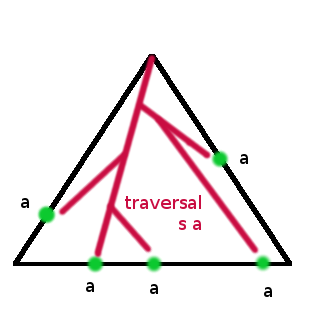
\includegraphics[scale=0.4]{traversal.png} 
\end{center}

Antwort: Wir bekommen eine \glqq \texttt{multi-lens}\grqq\ , genannt \texttt{Traversal}, mit mehreren Fokussen!

\end{frame}

%----------------------------------------------------------------------------------------

\begin{frame}[fragile]
\textbf{Ein Geständnis:}\dots\pause
Ich hab euch die ganze Zeit angelogen!\bigskip

\begin{minted}{haskell}
type Lens' s a = Lens s s a a

type Lens s t a b = forall f. Functor f =>
     (a -> f b) -> (s -> f t)
\end{minted}
\pause
\bigskip

\texttt{over} sieht auch nicht besser aus!

\begin{minted}{haskell}
over :: Profunctor p => Setting p s t a b
        -> p a b -> s -> t 
\end{minted}
\pause
\bigskip

\begin{center}
\glqq Edward is deeply in thrall to abstractionitis!\grqq\ (SPJ)
\end{center}

\end{frame}

%----------------------------------------------------------------------------------------

\begin{frame}

Es gibt natürlich noch mehr. Viel mehr.
\pause

\begin{itemize}
\item Prisms (indexed \texttt{Lens}es)
\item Rays (\texttt{Lens}es nach außen)
\item Generic Programming
\item Interaktionen mit \texttt{State}
\item \dots
\end{itemize}
\pause

Eventuell sehen wir davon noch ein paar Sachen in späteren Vorlesungen.\smallskip\smallskip

Die nach-Hause-Message ist, dass wir mit ein paar cleveren Typsysonymen und Typklassen in \texttt{Haskell} uns ein Framework basteln können, dass enorm viel Ausdruckskraft hat. \emph{The power of abstraction!}

\end{frame}

%----------------------------------------------------------------------------------------
\section{QuickCheck}
%----------------------------------------------------------------------------------------

\begin{frame}

\begin{center}
\Large
\textbf{QuickCheck\\(Randomised Property-Based Testing)}
\end{center}

\end{frame}

%----------------------------------------------------------------------------------------
\subsection{Motivation}
%----------------------------------------------------------------------------------------

\begin{frame}
\emph{Unit Testing} ist eine Vorgehensmethode in der Softwareentwicklung um Fehler
vorzubeugen bzw. früh zu finden (und bessere Dokumentation zu haben, oft auch besseres Design etc.).
\bigskip

Ein Entwickler schreibt zunächst \emph{Tests} (i.e. Code, der funktionieren \textit{sollte})
der Funktionalität benutzt, die noch nicht implementiert wurde, und gibt ein erwartetes
Ergebnis an. Bei jedem Build können diese Tests dann automatisch durchgeführt werden, um einen Überblick darüber zu erhalten, was funktioniert und was nicht.
\end{frame}

%----------------------------------------------------------------------------------------

\begin{frame}
\textbf{Types vs. Tests}\bigskip

\begin{wrapfigure}{r}{0.4\textwidth}
  \vspace{-20pt}
  \begin{center}
    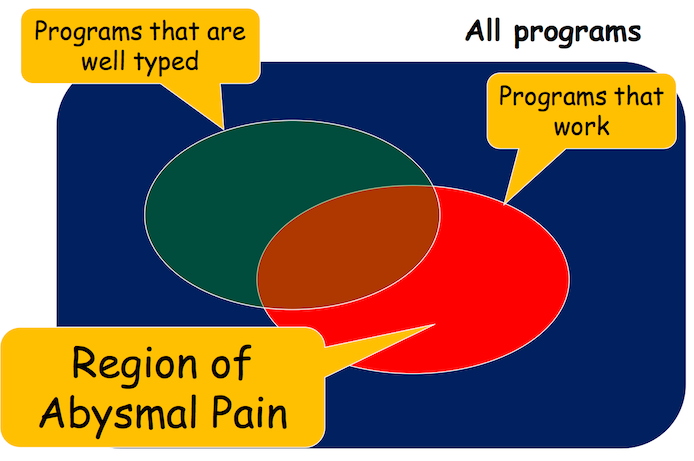
\includegraphics[scale=0.4]{region-of-abysmal-pain.png} 
  \end{center}
  \vspace{-20pt}
\end{wrapfigure}

In \texttt{Haskell} steht uns natürlich schon das Typsystem zur Seite, wenn es darum geht, korrekten Code zu schreiben. Und an vielen Stellen ist es auch sehr hilfreich, weil es viele Fehler bereits zur \emph{compile time} abfängt, die sonst in der \emph{run time} landen würden.
\bigskip

Allerdings ist das Typsystem von \texttt{Haskell} nicht stark genug, wirklich alle Fehler abzufangen. Oft genug kann man sich leicht dran vorbei schummeln.
\end{frame}

%----------------------------------------------------------------------------------------

\begin{frame}[fragile]

Man schaue sich die Typsignatur von \texttt{sort} (aus \texttt{Data.List}) an:

\begin{minted}{haskell}
sort :: Ord a => [a] -> [a]
\end{minted}

Alles, was wir wissen, ist, dass eine Liste von \texttt{a}s auf eine Liste von \texttt{a}s abgebildet wird. Mehr nicht.
\pause
\smallskip

Hier sind ein paar Implementationen, die erfolgreich typchecken:

\begin{minted}{haskell}
sort = const []
sort = id
sort = reverse
sort = \xs -> (permutations xs) !! 19
sort = take 5
\end{minted}
\pause

\dots und wenn diese Beispiele durchlaufen, dann auch euer beinahe-korrektes Programm mit einem kritischen off-by-one-error. Aber dafür sind Unit Tests gedacht!
\end{frame}

%----------------------------------------------------------------------------------------

\begin{frame}
Lesson learned: Unit Tests sind wichtig. Warum?\pause

Weil wir dumme, fehlbare, stolze Menschen sind!

\begin{center}
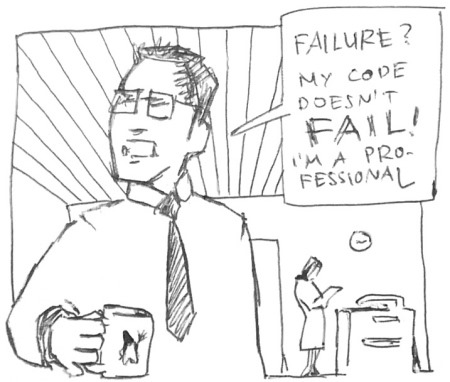
\includegraphics[scale=0.45]{unit_tests.jpg} 
\end{center}

\end{frame}

%----------------------------------------------------------------------------------------

\begin{frame}
\textbf{Das Problem mit Unit Tests}:
\bigskip

Wenn Unit tests also so toll sind, wo ist denn dann bitteschön die Problematik? Wir schreiben
die Tests, fertig aus. Wer braucht diese dumme Bibliothek?
\pause
\bigskip

Auch Unit Testing ist keine Silberkugel gegen Fehler in der eigenen Software:\pause

\begin{itemize}
\item Es ist eine Menge Arbeit, die signifikante Mengen an Zeit benötigt\pause
\item \dots es sei denn man macht es halbherzig. Dann verliert es aber seinen ganzen Sinn.\pause
\item Oft schreibt die Person, die ein Stück Code entwickelt auch die Tests für dieses Stück Code. Edge Cases, die eins hier übersieht, übersieht eins oft auch dort.\pause
\item \dots
\end{itemize}
\end{frame}

%----------------------------------------------------------------------------------------
\subsection{Idee und Anwendung}
%----------------------------------------------------------------------------------------

\begin{frame}
\textbf{Die Idee von QuickCheck: Automatisierte Testgenerierung}
\bigskip

Der große Sprung von QuickCheck ist, dass Menschen ihre Tests nicht mehr selbst schreiben,
sondern wir das einer Bibliothek überlassen. 
\pause 
\smallskip\smallskip

Um das zu ermöglichen (und das Testschreiben allen kürzer und einfacher zu machen), wechseln
wir von spezifischen Tests, die einzelne Werte überprüfen, zu \emph{property based testing}. Das bedeutet, dass wir im Code nur noch Eigenschaften formulieren, die unser Code haben soll.

\end{frame}

%----------------------------------------------------------------------------------------

\begin{frame}[fragile]

Ein paar Beispiele (zuerst \texttt{import Test.QuickCheck}):

\begin{itemize}
\item \texttt{reverse} doppelt angewendet hebt sich weg:
  \begin{verbatim}
  > quickCheck (\xs -> xs == (reverse . reverse) xs)
  +++ OK, passed 100 tests.
  \end{verbatim}
  \pause
\item Wenn $n$ gerade ist, ist $n+1$ ungerade (conditional):
  \begin{verbatim}
  > quickCheck(\n -> even(n) ==> odd(n+1))
  +++ OK, passed 100 tests.
  \end{verbatim}
  \pause
\item Früher wurde geglaubt, dass wenn $n$ prim ist, auch die $n$-te Mersenne-Zahl $\mathrm{M}_n = 2^n - 1$ prim ist.\\ (Die Vermutung hält für $\mathrm{M}_2$, $\mathrm{M}_3$, $\mathrm{M}_5$ und $\mathrm{M}_7$)
  \begin{verbatim}
  > quickCheck(\n -> isPrime n ==> isPrime(2^n - 1))
  *** Failed! Falsifiable (after 14 tests):                  
  11
  \end{verbatim}
\end{itemize}

\end{frame}

%----------------------------------------------------------------------------------------

\begin{frame}[fragile]

\begin{minted}{haskell}
-- Sorting twice changes nothing
prop_idempotency :: Ord a => [a] -> Bool
prop_idempotency xs = qsort xs == qsort (qsort xs)

-- Sorting doesn't change the length
prop_len :: Ord a => [a] -> Bool
prop_len xs = length xs == length (qsort xs)

-- Sorted result is a permutation of input
prop_perm :: Ord a => [a] -> Bool
prop_perm xs = (qsort xs) `elem` (permutations xs)

-- Sorting produces sorted list
prop_sort :: Ord a => [a] -> Bool
prop_sort = isSorted . qsort
  where
    isSorted :: Ord a => [a] -> Bool
    isSorted []       = True
    isSorted [x]      = True
    isSorted (x:y:zs) = (x <= y) && isSorted (y:zs)
\end{minted}

\end{frame}

%----------------------------------------------------------------------------------------

\begin{frame}[fragile]
Allerdings kann natürlich auch QuickCheck reingelegt werden. Und 100 Test Cases sind 
bei weitem nicht immer genug:
\pause

\begin{verbatim}
> let notProduct n p q = n /= p * q
> quickCheck (notProduct 10)
+++ OK, passed 100 tests.
> quickCheck (notProduct 10)
+++ OK, passed 100 tests.
> quickCheck (notProduct 10)
+++ OK, passed 100 tests.
> quickCheck (notProduct 10)
*** Failed! Falsifiable (after 9 tests):                  
5
2
\end{verbatim}
\pause

Es kommt leider immer noch auf die Person vor der Tastatur an.
\end{frame}

%----------------------------------------------------------------------------------------

\begin{frame}
Lesson learned: Unit Tests zu automatisieren wichtig. Warum?\pause

Weil wir dumme, fehlbare, stolze Menschen sind!

\begin{center}
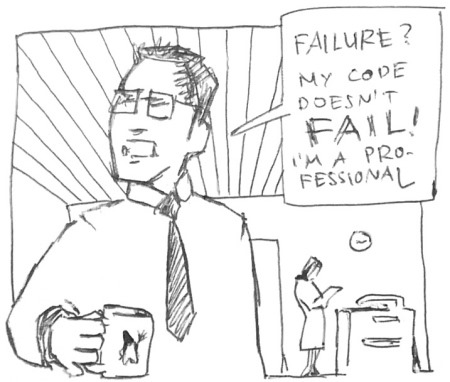
\includegraphics[scale=0.45]{unit_tests.jpg} 
\end{center}

\end{frame}

%----------------------------------------------------------------------------------------


\end{document}
